\documentclass[12pt]{article}
\usepackage[english]{babel}
\usepackage[utf8x]{inputenc}
\usepackage[T1]{fontenc}
\usepackage{scribe}
\usepackage{listings}
\usepackage{graphics, graphicx}
\usepackage{enumitem}
\usepackage{tcolorbox}
\usepackage{adjustbox}
\usepackage[ruled,vlined]{algorithm2e}



\graphicspath{ {./images/} }

\CourseName{Comtemporary Algorithms T.II/2019-20}
\Scribe{Suchanun P.\& Suchanuch P.}
\Lecturer{Dr. Kanat Tangwongsan}
\LectureNumber{10}
\LectureDate{5 February 2020}
\LectureTitle{Parallel Algorithms IV}

\lstset{style=mystyle}

\newlist{steps}{enumerate}{1}
\setlist[steps, 1]{label = Step \arabic*:}

\begin{document}
\MakeScribeTop

\section{Prime Sieves}

\subsection{Finding primes $\leq$ n}

$is\_prime(x)$ returns whether or not $x$ is prime.\\
Sequential: $W = O(\sqrt{x})$\\
Parallel: $W = O(\sqrt{x}), S = O(\log x)$\\ \\
$find\_primes$ returns all primes up to $n$.

\begin{algorithm}[H]
\SetAlgoLined
 \For{i in range(2, n+1)}{
  flags[i] = $\textrm{is\_prime}(i)$\;
 }
 \Return flags.filter(lambda x: x)  \tcp*{where flags store $True$}
 \caption{find\_primes(n)}
\end{algorithm}
$W = O(n\sqrt{n})$ and 
$S =O(\log n)$

\subsection{Sieve of Eratosthenes}

To find all primes up to $n$. Generate a list of integers from $2$ to $n$. Say $n=30$


\includegraphics[scale=0.5]{img0}

The first number in the list is $2$. Cross out all multiple of 2 from the list.


\includegraphics[scale=0.5]{img1}

The next number in the list is $3$. Cross out all its multiple from the list.

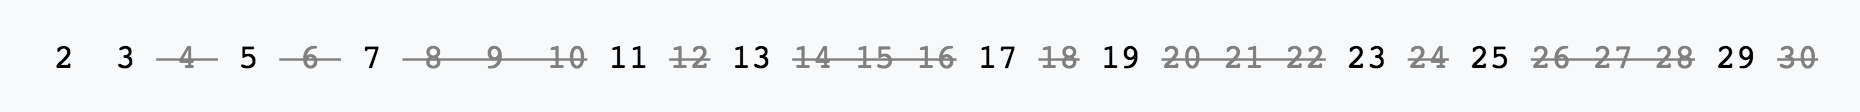
\includegraphics[scale=0.5]{img2}

The next number not yet crossed out in the list after 3 is 5. 

Repeat the same process until we cross the multiples of $\sqrt{n}$


\includegraphics[scale=0.5]{img3}

\clearpage

The numbers not crossed out at this point are all primes.

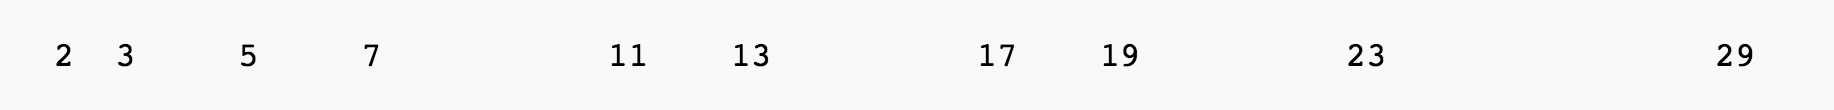
\includegraphics[scale=0.5]{img4}

$T = \sum_{p=primes\leq n} \frac{n}{p} \leq n(\log \log n + const) = O(n \log \log n)$  

\begin{algorithm}[H]
\SetAlgoLined
 \If {n<2}{
 	\Return []
 	}
 sqrtn = sqrt(n)\;
 low\_primes = find\_primes(sqrtn)  \tcp*{$W: O(\sqrt{n}),\textrm{\ }S: O(\sqrt{n})$}
 flags = [True]*n\;
 $\textbf{p}$\For( \tcp*[f]{$W: O(n\log \log n),\textrm{\ }S: O(1)$}){p in lowprimes}{ 
 	$\textbf{p}$\For{(i = $\textrm{sqrtn/p}$; i< n/p; i++)}{
 		flags[$p*i$] = False\;
 	}
 }
	high\_primes = filter(range(sqrt+1, n+1), lambda x: flags[x]) \tcp*{$W: O(n),\textrm{\ } S: O(\log {n})$}
 \Return low\_primes + high\_primes
 \caption{find\_primes(n)}
\end{algorithm}
\textbf{Work and Span}\\
$W(n) = W(\sqrt{n}) + O(n \log \log n) = O(n \log \log n)$\\
$S(n) = S(\sqrt{n}) + O(\log n) = \log n + \frac{1}{2}\log n + \frac{1}{4} \log n + \ldots = O(\log n)$ 

\section{MST}
Given $(V, E, w)$, get MST of minimum weight.\\
Boruvka (1926) - based on Light Edge Rule\\
\textbf{Theorem:} Let $G = (V,E,w)$ be a connected, undirected graph qith distinct edge weights. For any nonempty $U \subset V,$ the minimum weight edge between $U$ and $V \setminus  U$ is in the $MST$ of $G$.\\
\textbf{Observation}: The min edge of each vertex appears in the $MST$.\\
\textbf{Claim1}: The min edge form a forest (with no cycles)\\
\textbf{Claim2}: \# nodes contracted $\geq \frac{n}{2}$

\begin{algorithm}[H]
\SetAlgoLined
 \If {$|V|==1$}{
 	\Return \;
 	}
 every vertex picks its min edge $\rightarrow$ mindEdges; add this to final MST\tcp*{$W:O(n)\textrm{\ } S: O(1)$}
 run tree-contract on minEdges $\rightarrow G' = (V', E')$, \tcp*{$W:O(m),\textrm{\ } S: O(\log ^2 n)$}
 MST(G') \tcp*{$W: \leq W(\frac{n}{2}, m),\textrm{\ } S: S(\frac{n}{2},m)$}
 \caption{MST($G = (V,E))$}
\end{algorithm}
\textbf{Work and Span}\\
$W(n, m) \leq W(\frac{n}{2}, m) + O(n) + O(m) \leq O(m \log n +n)$\\
$S(n,m) = S(\frac{n}{2}, m) + O(\log^2 n) = O(\log ^3 n)$

\section{Connectivity}
Given $G = (V, E)$, want to assign labels $l: v \rightarrow \{0,...\}$, \\
such that $l(u) = l(v) \rightarrow u$ is connected to $v$.\\

\textbf{Sequencial BFS/DFS }can do this in $O(m+n)$.

\subsection{Low-diameter decomposition}
Goal: decompose V into a set of clusters s.t.\\
	1. the number of inter-cluster edges is “small”\\
	2. diameter of each cluster is “small” (~log(n)) \\
	
\textbf{Def: } a $(\beta,d)-$decomposition, $0 < \beta < 1$, is a partition of $V$ into $V_1, V_2, ..., V_k$ such that
\begin{itemize}
	\item total number of edges across components $\leq \beta m$ (few inter-component edges)
	\item the shortest path between any 2 vertices in  $u, v \in V_i$, using only vertices in $V_i$ is at most $d$. (strong diameter) 
\end{itemize}
	
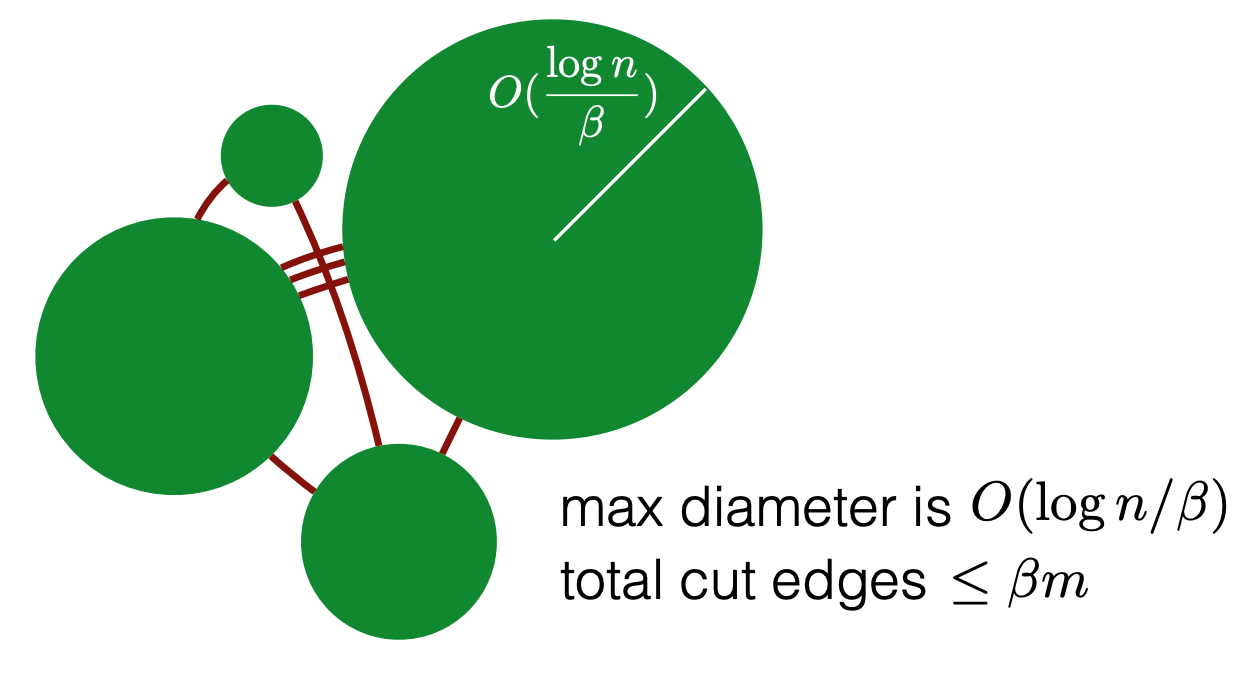
\includegraphics[scale=0.5]{mpx}

\textbf{Theorem: } Parallel low-diameter decomposition can find $(\beta, d)-$ decomposition 

where  $\beta \leq 1/2$ and $d \in O(\log n/\beta)$ in $O(m)$ work and $O(\log ^2n)$ span with high probability.

\end{document}
